\documentclass[12pt,a4paper,openright,twoside]{book}
\usepackage[utf8]{inputenc}
\usepackage{disi-thesis}
\usepackage{code-lstlistings}
\usepackage{notes}
\usepackage{shortcuts}
\usepackage{acronym}

\school{\unibo}
\programme{Corso di Laurea in Ingegneria e Scienze Informatiche}
\title{Sistema di visione
	artificiale per la rilevazione e posa di
	marker ArUco sviluppato in Java}
\author{Bacchini Lorenzo}
\date{\today}
\subject{Programmazione ad oggetti}
\supervisor{Prof. Mirko Viroli}
\cosupervisor{Dott. Gianluca Aguzzi}
\morecosupervisor{Dott. Nicolas Farabegoli}
\session{III}
\academicyear{2023-2024}

% Definition of acronyms
%\acrodef{IoT}{Internet of Thing}
%\acrodef{vm}[VM]{Virtual Machine}


\mainlinespacing{1.241} % line spacing in mainmatter, comment to default (1)

\begin{document}

\frontmatter\frontispiece

\begin{abstract}	
Max 2000 characters, strict.
\end{abstract}

\begin{dedication} % this is optional
Optional. Max a few lines.
\end{dedication}

%----------------------------------------------------------------------------------------
\tableofcontents   
\listoffigures     % (optional) comment if empty
\lstlistoflistings % (optional) comment if empty
%----------------------------------------------------------------------------------------

\mainmatter

%----------------------------------------------------------------------------------------
\chapter{Introduction}
\label{chap:introduction}
%----------------------------------------------------------------------------------------

Write your intro here.
\sidenote{Add sidenotes in this way. They are named after the author of the thesis}

You can use acronyms that your defined previously,
such as \ac{IoT}.
%
If you use acronyms twice,
they will be written in full only once
(indeed, you can mention the \ac{IoT} now without it being fully explained).
%
In some cases, you may need a plural form of the acronym.
%
For instance,
that you are discussing \acp{vm},
you may need both \ac{vm} and \acp{vm}.

\paragraph{Structure of the Thesis}

\note{At the end, describe the structure of the paper}

\chapter{Background}

\section{Visione artificiale}

\subsection{Cos'è la visione artificiale?}
Quando parliamo di visione artificiale o computer vision stiamo considerando un insieme di processi e tecniche che hanno come scopo finale quello di trasformare degli input (solitamente foto o video \footnote{gli input potrebbero essere anche generati da scanner, sensori LiDaR, radar ecc.}) in una serie di informazioni utili al calcolatore che possono poi essere utilizzate per prendere decisioni in maniera autonoma, analizzare una situazione o addirittura creare una rappresentazione del mondo reale 3D che ci circonda. \cite{bradski2008learning} \cite{microsoftArtificialVision}

Quanto sopra descritto non è troppo diverso da ciò che i nostri occhi fanno tutti i giorni, ed infatti la visione artificiale nasce proprio per permettere al calcolatore di "vedere" esattamente come un essere umano, in modo da poter interagire con l'ambiente circostante.

\subsection{Come funziona la visione artificiale?}
Il processo di visione artificiale può essere suddiviso tre fasi principali:
\begin{enumerate}
	\item Rilevazione di un immagine
	\item Interpretazione e analisi dell'immagine
	\item Richiesta di informazioni sull'immagine analizzata
\end{enumerate}
Nella fase di rilevazione come sopra citato è possibile utilizzare diversi tipi di strumenti come fotocamere o videocamere, ma è nella fase centrale che il processo può differire maggiormente, infatti, l'interpretazione dell'immagine viene effettuata secondo algoritmi che possono essere anche molto diversi in base al loro scopo, negli ultimi anni inoltre si stanno facendo largo nuove tecnologie \footnote{con il termine nuove non si intende che tecnologie come l'intelligenza artificiale o il machine learning siano state sviluppate negli ultimi anni ma che iniziano ad essere prese sempre più in considerazione nell'ambito della visione artificiale} come l'intelligenza artificiale, il machine learning e il deep learning per poter intraprendere decisioni e svolgere compiti in modo autonomo senza il bisogno dell'intervento umano.

\subsection{Applicazioni e finalità}
Alcune applicazioni della visione artificiale sono le seguenti:
\begin{itemize}
	\item Classificazione di immagini
	\item Identificazione di oggetti
	\item Suddivisione di immagini in sezioni da analizzare
	\item Riconoscimento facciale
	\item Rilevazione e riconoscimento dei sentimenti in una immagine
	\item Ricostruzione di ambienti 3D
	\item Guida autonoma
\end{itemize}
La lista dei possibili utilizzi è ovviamente molto vasta ma quelli riportati sopra sono tra i più gettonati sia in ambito professionale che di ricerca.

\subsection{Principali criticità}
Tutte le operazioni che caratterizzano un sistema di visione artificiale possono essere largamente influenzate da una serie di condizioni interne o esterne con il risultato che il nostro sistema potrebbe non operare come previsto.

Un esempio di condizioni esterne che possono influenzare il comportamento del nostro sistema sono sicuramente l'illuminazione, la prospettiva ed eventuali occlusioni dell'immagine in input, che possono portare ad una maggiore difficoltà di rilevazione e riconoscimento, per quanto riguarda invece i parametri interni possiamo considerare la risoluzione della camera che stiamo utilizzando, l'algoritmo di elaborazione e la complessità (in termini numero di pixel da elaborare) dell'immagine ottenuta, come parametri che possono variare anche di molto la velocità e la precisione del nostro sistema.

\subsection{Cenni storici}
I primi articoli prodotti riguardanti la visione artificiale risalgono agli anni '60 dove però l'idea di poter acquisire immagini ed elaborarle, facendone comprendere il contenuto all'elaboratore era ancora troppo precoce per l'hardware a disposizione,
solo intorno agli anni '80 si sono iniziati a vedere i primi sviluppi significativi grazie all'introduzione della \href{https://en.wikipedia.org/wiki/Hough_transform}{trasformata di Hough}
e dei primi algoritmi di riconoscimento ottico dei caratteri (OCR - optical character recognition).
Dagli anni '90 sino ai primi anni '00 l'attenzione si è spostata sullo sviluppo di algoritmi di machine learning, questo ha permesso nel 2001 di sviluppare il primo algoritmo di riconoscimento facciale.\cite{artificialVisionHistory}

Ad oggi la visione artificiale adotta tecniche e processi completamente differenti rispetto a quelli visti nei suoi primi anni di sviluppo, facendo largo uso di reti convoluzionali e dell'intelligenza artificiale (ormai largamente utilizzabile grazie alla sempre crescente potenza di calcolo a disposizione) che le permettono non solo di essere più veloce ma anche di garantire una precisione dei risultati molto maggiore grazie anche al vasto numero di dati a disposizione.

\section{Marker fiduciali}
\subsection{ArUco markers}

\section{OpenCV}

\chapter{Analisi}

\chapter{Design}

\chapter{Implementazione}

\chapter{Valutazione}

\chapter{Conclusioni}

\chapter{Sviluppi futuri}

\chapter{Ringraziamenti}

I suggest referencing stuff as follows: \cref{fig:random-image} or \Cref{fig:random-image}

\begin{figure}
    \centering
    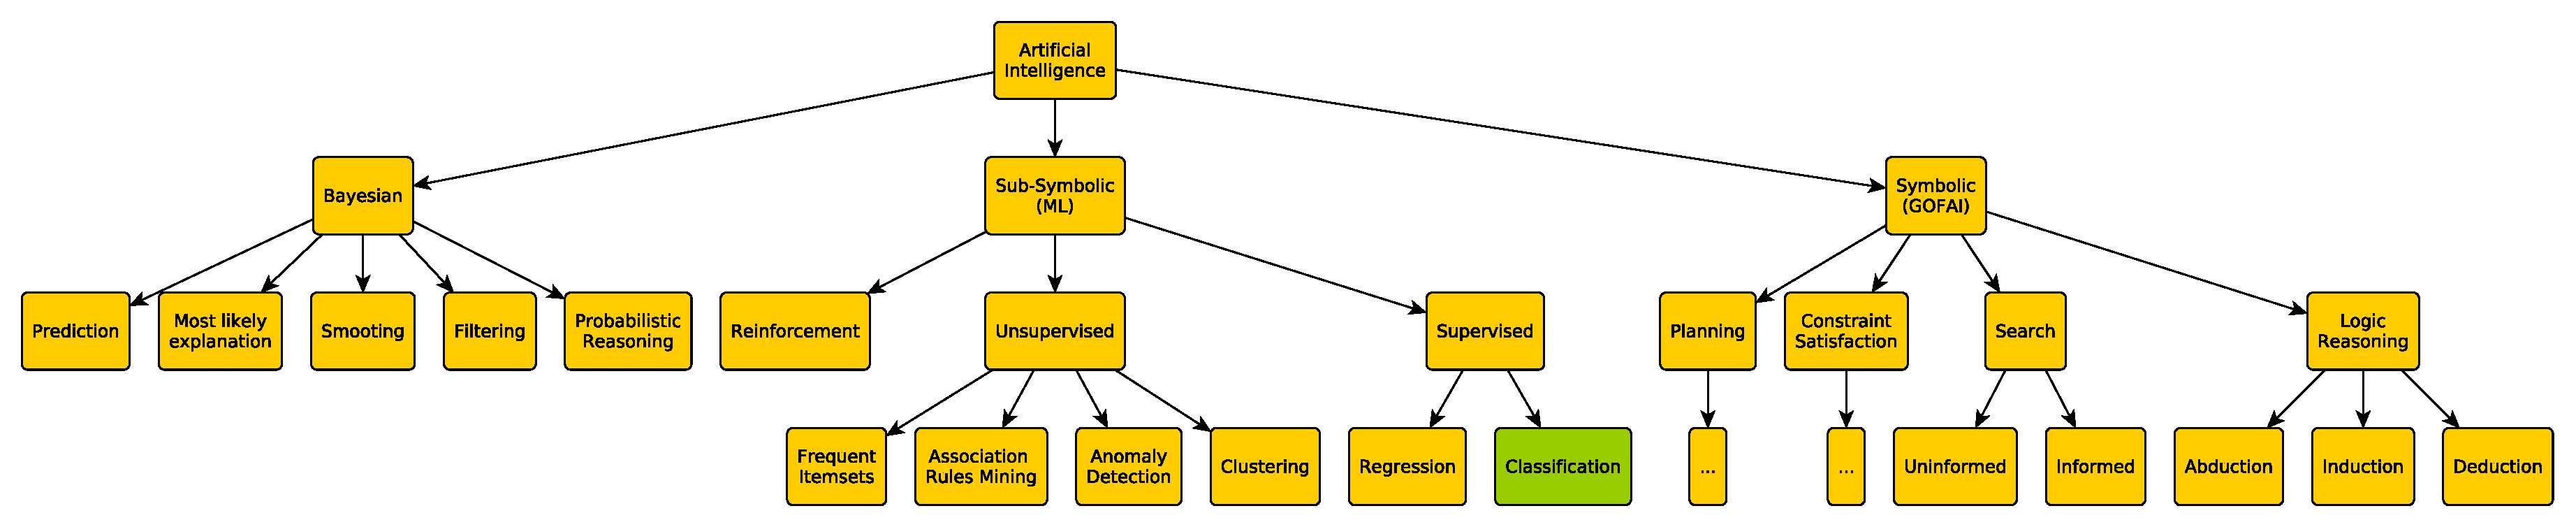
\includegraphics[width=.8\linewidth]{figures/random-image.pdf}
    \caption{Some random image}
    \label{fig:random-image}
\end{figure}

\section{Some cool topic}

\chapter{Contribution}

You may also put some code snippet (which is NOT float by default), eg: \cref{lst:random-code}.

\lstinputlisting[float,language=Java,label={lst:random-code}]{listings/HelloWorld.java}

\section{Fancy formulas here}

%----------------------------------------------------------------------------------------
% BIBLIOGRAPHY
%----------------------------------------------------------------------------------------

\backmatter

\nocite{*} % Remove this as soon as you have the first citation

\bibliographystyle{alpha}
\bibliography{bibliography}

\begin{acknowledgements} % this is optional
Optional. Max 1 page.
\end{acknowledgements}

\end{document}
